\chapter{Data Representation}

\begin{itemize}
	\item By \textbf{correlation}\\ 
   I want to represent data according to the correlation of the dataset\\
Algorithm: \texttt{PCA}
	\item By \textbf{neighborhood}\\ I want to represent the data so that similar instances are similar\\
Algorithm: \texttt{t-SNE}
	\item By \textbf{manifold}\\ 
   I want to represent the data so that its manifold is preserved\\
Algorithm: \texttt{UMAP}
\end{itemize}


\section{Principal Component Analysis (PCA)}

PCA is a linear dimensionality reduction technique
that transforms the data to a new coordinate system such that the greatest variance by any projection of the data comes to lie on the first coordinate (called the first principal component), the second greatest variance on the second coordinate, and so on.

Essentially, PCA exploits spectral decomposition of the whole dataset to find a new basis for the data.

Data can often be correlated, and linear dependencies can exist among variables,
e.g.,
\begin{itemize}
	\item Rent is linearly dependent on salary and food expenses
	\item Bank deposit is linearly dependent on salary and work
	\item Cardio is linearly dependent on $VO_2 max$
\end{itemize}

Vectors are $m$-dimensional elements in a field, and enjoy both addition and multiplication by scalar.\\ Composing these two, we can generate an infinite number of vectors: this is a \textbf{vector space}, and is defined by the basis vectors involved in the composition.

\begin{figure}[htbp]
   \centering
   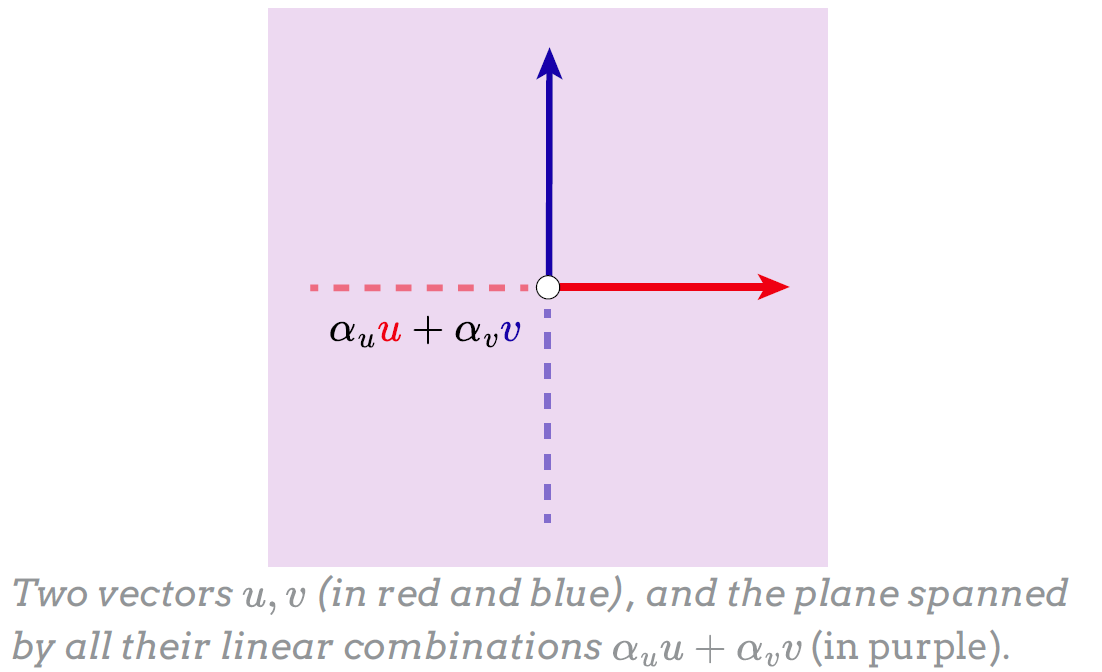
\includegraphics{images/02/span.png}
   \caption{Vector space spanned by two vectors}
   \label{fig:02/span}
\end{figure}

A matrix $A$ defines a space\dots and thus a linear
transformation! $Av$ linearly combines the columns of
with coefficients given by $v$.

\begin{paracol}{2}
   
   Eigenpairs $(\lambda, v)$ of a square matrix $A$ are defined by the equation $Av = \lambda v$.
   
   The eigenvectors $v_1,\dots,v_m$ of a matrix $A$ define the stretching of the space, and
   their eigenvalues $\lambda_1 > \dots > \lambda_m$ define the stretching factor.

   \switchcolumn

   \begin{figure}[htbp]
      \centering
      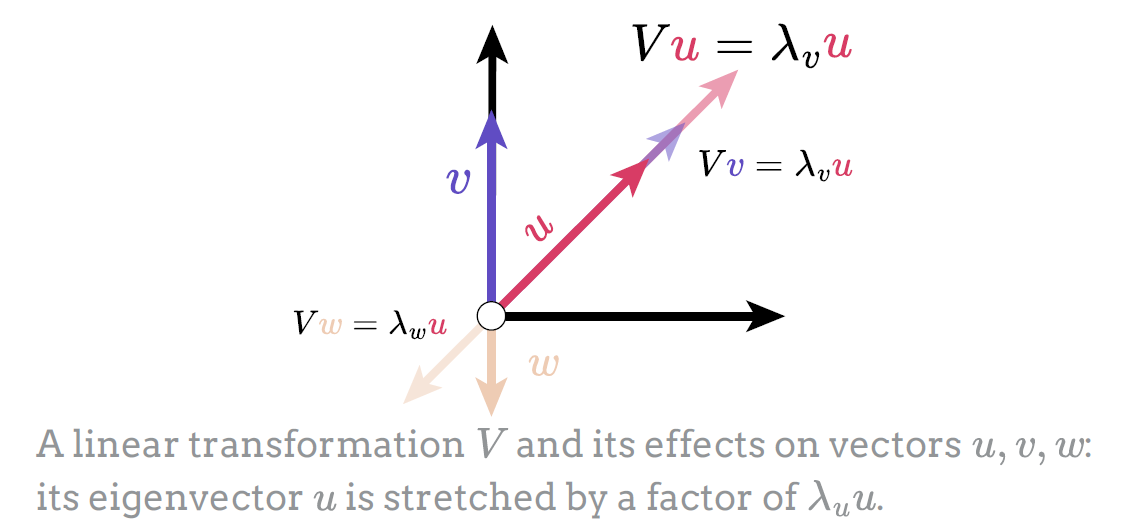
\includegraphics{images/02/eigenvector.png}
      \caption{Eigenvectors of a matrix}
      \label{fig:eigenvector}
   \end{figure}
\end{paracol}

% Bla about matrices skipped

PCA projects some data $X$ to $\hat{X}$ through a linear transformation $A$: $AX = \hat{X}$.

Fun fact \#1: for a mean-centered $\bar{X}$, the slope is directly proportional to the covariance!

\[
\bar{\Sigma} = \begin{bmatrix}
\sigma_{\bar{X}^1}^2 & \cdots & \text{cov}(\bar{X}^1, \bar{X}^n) \\
\cdots & \cdots & \cdots \\
& & \sigma_{\bar{X}^n}^2
\end{bmatrix}
\]

%PCA notes

% TODO various notes fino a slide 25

There is some pretty complicated linear algebra behind PCA, but the main steps are the following:
\begin{enumerate}
   \item Mean-center your data $X$ to get $\bar{X}$
   \item Compute its eigenvectors matrix $\bar{V}$
   \item Transpose $V$ to obtain the transformation $V^T$
   \item Project the data: $\bar{X}$ through $V^T\bar{X}$, obtaining the PCA-transformed data $\hat{X}$ 
\end{enumerate}

\textbf{In simple terms:} PCA looks at your data and finds the ``most important directions" - imagine you have a cloud of points and you want to find the best line that captures the main trend. PCA finds not just one line, but multiple directions ordered by importance. It then rotates your data so that the first dimension captures the most variation, the second dimension captures the second most variation. This allows you to keep only the first two dimensions while retaining most of the information, effectively reducing the complexity of your data while preserving its essential structure.

\subsection{Observations}
\begin{itemize}
	\item PCA redefines data by removing
collinearity: if your data has low
covariance, the transformation will
have minimal effect.
	\item PCA performs a linear
transformation to tackle linear
relationships between variables.
Nonlinear relationships are not
influenced.
   \item PCA does not work very well for high complexity data.
\end{itemize}

\labelitemize{\textit{Uses}}{
  \begin{itemize}
  	\item \textbf{Feature selection}: high covariance
  	      of a feature may indicate
  	      disposability.
  	\item \textbf{Dimensionality reduction}:
  	      trimming columns of lets us
  	      reduce the dimension of the
  	      resulting data.
  	\item \textbf{Clustering preprocessing}:
  	      correlated features inflate object
  	      similarity
  \end{itemize}
}

\section{t-SNE}
t-SNE (t-distributed Stochastic Neighbor Embedding) is a nonlinear dimensionality reduction technique particularly well suited for embedding high-dimensional data for visualization in a low-dimensional space of two or three dimensions. It works by modeling the data as a distribution of points in a high-dimensional space and then finding a lower-dimensional representation that preserves the pairwise similarities between points.



\texttt{t-SNE} focuses on data clusters rather than subspace representation, and again maps the original data $X$ to a representation $\hat{X}$.

{\texttt{t-SNE} tackles this problem in two phases:\ns
\begin{enumerate}
   \item \textbf{Similarity phase} In the original space $\mathcal{X}$, how similar is $x_i$ to $x_j$?
   \note{How similar is $x_i$ to $x_j$? Even better, what is the probability that $x_i$ is a neighbor of $x_j$?}
   
   \item \textbf{Embedding phase} In the mapped space $\hat{\mathcal{X}}$, how similar is $\hat{x}_i$ to $\hat{x}_j$?
\end{enumerate}
}

\subsection{Similarity phase}
\begin{figure}[htbp]
   \centering
   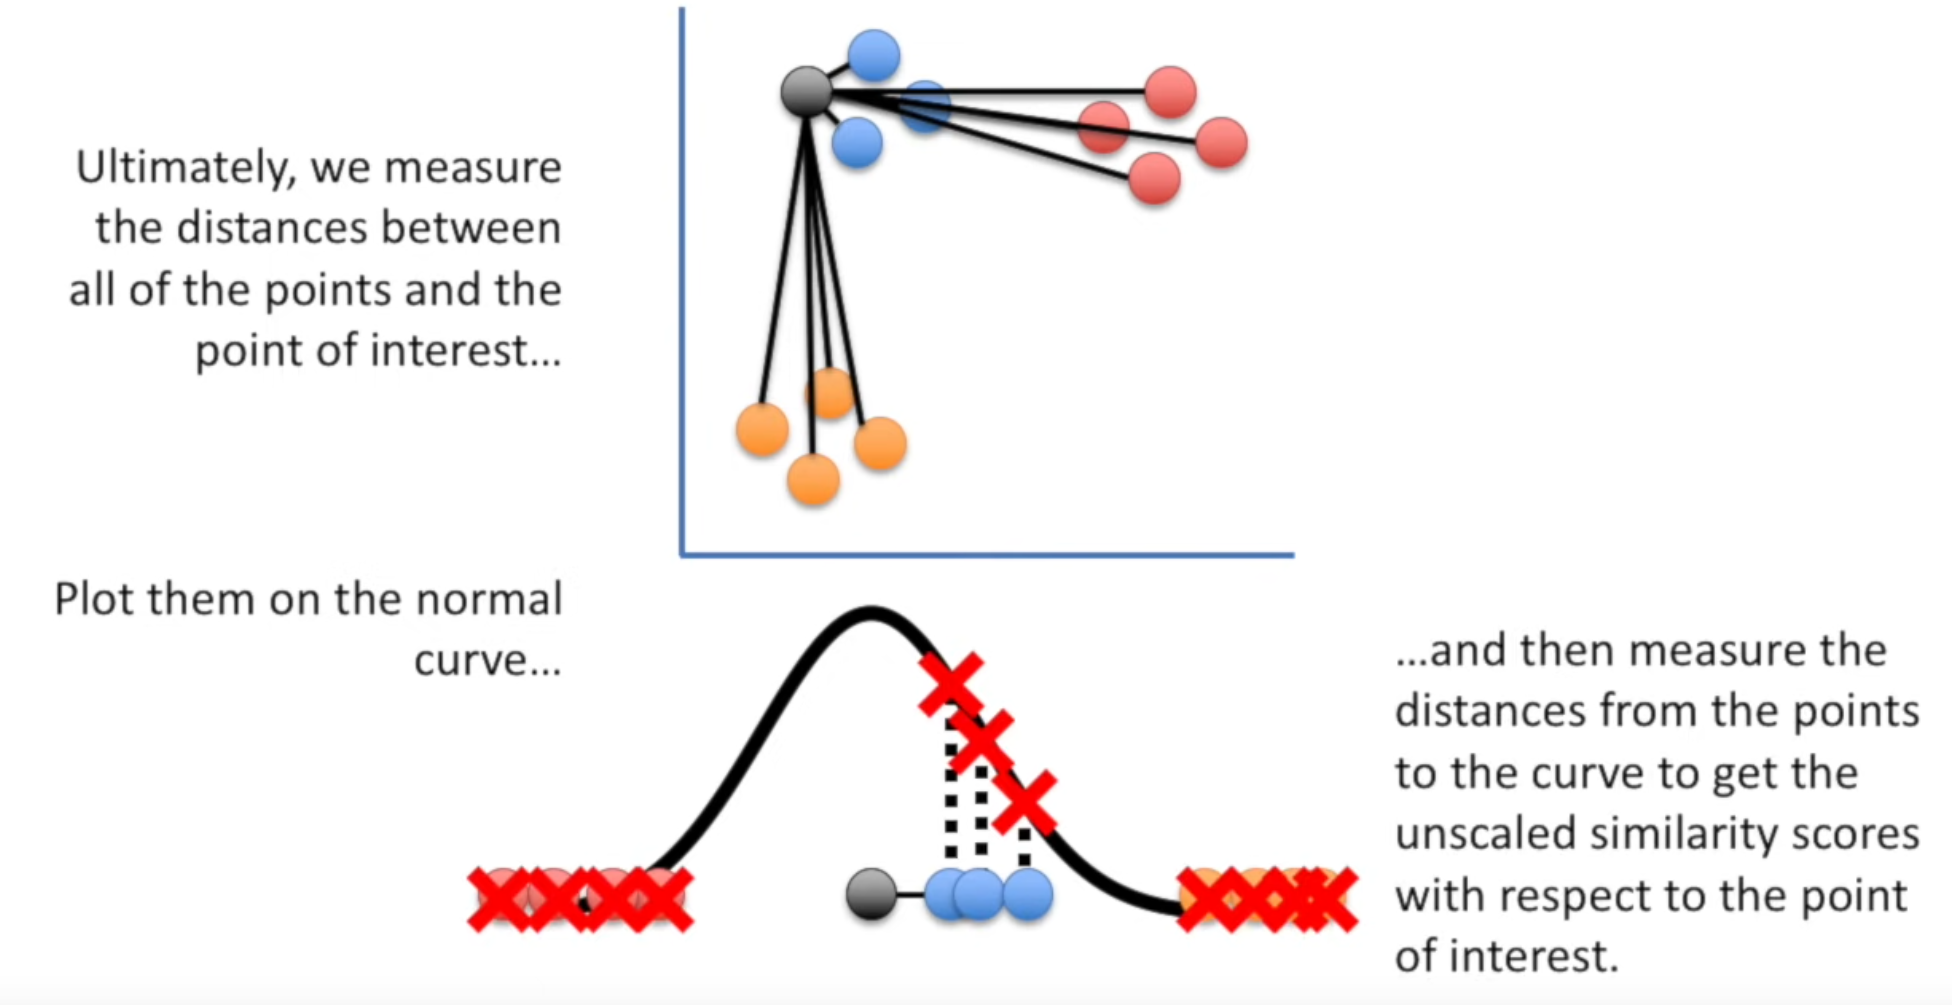
\includegraphics{images/02/tsne.png}
   \caption{t-SNE plotting distance on an X axis and then projecting it on a normal distribution curve, to get the probability of being a neighbor}
   \label{fig:02/tsne}
\end{figure}
The similarity phase computes the similarity between points in the original high-dimensional space. This is typically done by converting the Euclidean distances between points into conditional probabilities that represent similarities. The probability that point $x_j$ is a neighbor of point $x_i$ is given by a Gaussian distribution centered at $x_i$. The variance of this Gaussian is controlled by a parameter called \textbf{perplexity}, which can be thought of as a smooth measure of the effective number of neighbors.

This yields a neighboring matrix $P$ where each entry $p_{ij}$ represents the probability that point $x_j$ is a neighbor of point $x_i$ in the original high-dimensional space.

The conditional probability is computed as:
\[
p_{j|i} = \frac{\exp(-||x_i - x_j||^2 / 2\sigma_i^2)}{\sum_{k \neq i} \exp(-||x_i - x_k||^2 / 2\sigma_i^2)}
\]

where $\sigma_i$ is the variance of the Gaussian centered at point $x_i$. The perplexity parameter determines $\sigma_i$ through a binary search to match the desired effective number of neighbors.

\subsection{Embedding phase}

In the embedding phase, t-SNE defines a similar probability distribution over the points in the low-dimensional map. However, instead of using a Gaussian distribution, it uses a Student's t-distribution with one degree of freedom (heavy-tailed distribution) to avoid the ``crowding problem" where moderate distant points are forced to be too far apart in the low-dimensional representation.

The probability in the low-dimensional space is:
\[
q_{ij} = \frac{(1 + ||y_i - y_j||^2)^{-1}}{\sum_{k \neq l} (1 + ||y_k - y_l||^2)^{-1}}
\]

where $y_i$ and $y_j$ are the low-dimensional counterparts of $x_i$ and $x_j$.

\subsection{Optimization}

t-SNE minimizes the Kullback-Leibler divergence between the probability distributions $P$ (high-dimensional) and $Q$ (low-dimensional):

\[
C = \sum_i KL(P_i||Q_i) = \sum_i \sum_j p_{j|i} \log \frac{p_{j|i}}{q_{j|i}}
\]

The algorithm uses gradient descent to find the low-dimensional representation $Y$ that minimizes this cost function, effectively preserving the neighborhood structure of the original high-dimensional data.

\textbf{Key advantages:}
\begin{itemize}
	\item Excellent for visualization of high-dimensional data
	\item Preserves local neighborhood structure
	\item Can reveal clusters and patterns not visible in linear methods
\end{itemize}

\textbf{Key limitations:}
\begin{itemize}
	\item Computationally expensive (quadratic in the number of points)
	\item Non-deterministic (different runs can give different results)
	\item Sensitive to hyperparameters, especially perplexity
	\item Not suitable for embedding new data points (no explicit mapping function)
\end{itemize}

\section{UMAP}

UMAP (Uniform Manifold Approximation and Projection) is a nonlinear dimensionality reduction technique that is particularly effective for visualizing high-dimensional data in a low-dimensional space. It is based on manifold learning and topological data analysis, aiming to preserve both local and global structure of the data.

The computed distances induce a connectivity graph, and thus an adjacency matrix $A$,
its edges measuring distances among instances. After turning distances into
probabilities, UMAP optimizes a distance on $A$, to make it so that all and only the edges
on the original manifold also appear in the transformed manifold with the same
magnitude.

For the set of edges $E$, UMAP minimizes
\[
-\sum_{e \in E} \left( \underbrace{\Pr(e; X) \log(\Pr(e; Z))}_{\text{existing edges}} + \underbrace{(1 - \Pr(e; Z)) \log(1 - \Pr(e; X))}_{\text{non-existing edges}} \right),
\]

where $\Pr(e; X), \Pr(e; Z)$ indicate the probability of edge $e$ in the original and transformed representation, respectively.
